\chapter{Dataset} \label{dataset}
Dataset is very important for the training. Sufficient data that meets the requirement of the task is crucial, and the proper preprocessing can effectively help the model learn well. Based on the complexity of the indoor environment, which leads to the wide dynamic range of the data amplitude, we choose to collect the required dataset by ourselves so that the model can better adapt to complex range-Doppler map.

\section{Dataset recording} \label{dataset recording}
% The hardware of the radar product, the parameters, settings of recording, the environment and environment split, and the size of the dataset as well as resampling.

\begin{spacing}{1.5}
\textbf{\large{Radar hardware}}
\end{spacing}

In the collection of the dataset, we used the type of BGT60TR13C radar from Infineon \cite{ag_bgt60tr13c_nodate}. The BGT60TR13C type is a 60 GHz radar sensor with four integrated antennas, which includes single \gls{tx} and three \glspl{rx}, where the receivers are arranged in L-shape as shown in Figure \ref{the antenna arrangement of the radar}. In the task, due to the single channel chirp sequence radar, one of the three receivers has to be chosen. \gls{rx}3 is used by default during the recording, since \gls{rx}1 and \gls{rx}2 are closer to the \gls{tx} than Rx3, it means that the interference between signals will increase, and the noise will increase accordingly. On the other hand, using different receivers can increase the variety of data to a certain extent, so \gls{rx}1 is also sometimes used in the collection process.

\begin{figure}
	\centering
	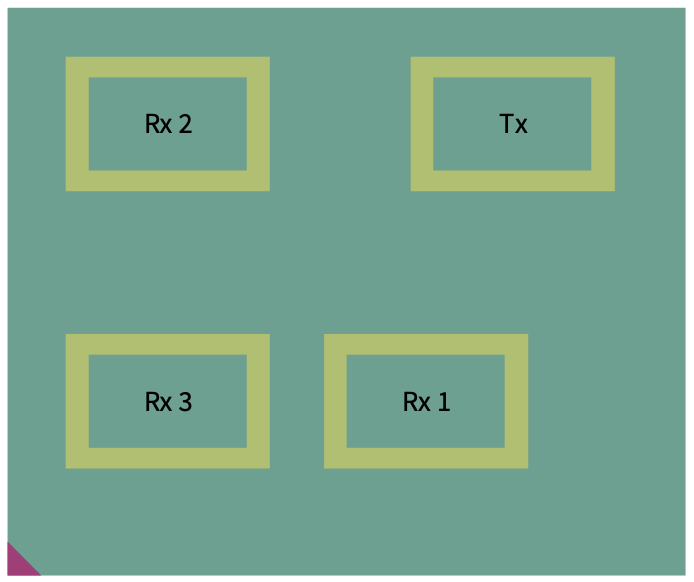
\includegraphics[scale=.5]{thesis/figures/antenna arrangement.png}
	\caption{The antennas arrangement of the radar device \cite{ag_bgt60tr13c_nodate}}
	\label{the antenna arrangement of the radar}
\end{figure}

The advantage of the BGT60TR13C radar is that it can achieve ultra-wide bandwidth \gls{fmcw} operation in a small package, which is conducive to provide higher resolution, retain more details and provide more possibilities in data, such as the downsample as the factor of 4. With a bandwidth of 5.5 GHz, the minimum range resolution is \SI{3}{\centi\meter}. Furthermore, the high \gls{snr} of this radar can achieve detection of up to \SI{15}{\meter}, providing a good hardware foundation for the movement, identification and segmentation of objects within this range, where more parameters are given in Table \ref{parametrics of the radar product}.

\begin{table}
    \centering
    \caption{Parameters of the BGT60TR13C radar product \cite{ag_bgt60tr13c_nodate}}
    \label{parametrics of the radar product}
    \begin{tabular}{cc|cc}
        \hline
        \multicolumn{1}{l|}{Parametrics} & BGT60TR13C & \multicolumn{1}{l|}{Parametrics} & BGT60TR13C \\
        \hline
        \multicolumn{1}{l|}{Angle of Arrival} & Yes & \multicolumn{1}{l|}{Current consumption} & 200 mA \\
        \hline
        \multicolumn{1}{l|}{Motion} & Yes & \multicolumn{1}{l|}{Supply voltage} & 1.8 V \\
        \hline
        \multicolumn{1}{l|}{Frequency} & 60 GHz & \multicolumn{1}{l|}{Gain} & 5 dBi \\
        \hline
        \multicolumn{1}{l|}{Min. frequency} & 58 GHz & \multicolumn{1}{l|}{Max detection range} & 15 m \\
        \hline
        \multicolumn{1}{l|}{Max. frequency} & 63.5 GHz & \multicolumn{1}{l|}{Min detection range} & 0.2 m \\
        \hline
        \multicolumn{1}{l|}{Range} & Yes & \multicolumn{1}{l|}{Speed} & Yes \\
        \hline
        \multicolumn{1}{l|}{Number of Rx antennas} & 3 & \multicolumn{1}{l|}{Number of Tx antennas} & 1 \\
        \hline
        % \multicolumn{1}{l|}{Minimal required TX power ($\mu \mathrm{W}$)} & 0.99 & 1.91 & 2.49 & 2.94 & 4.32\\
    \end{tabular}
\end{table}

While using this BGT60TR13C radar, Infineon provides a corresponding radar \gls{sdk}, which can access radar sensors and collect data through C/C++, Python and MATLAB, and can implement some radar algorithms such as range-Doppler map, simple segmentation, etc. with the \gls{sdk}. In addition, Infineon also provides wrappers that adapt to multiple platforms, such as MacOS, Linux, etc. For specific instructions, the developer community and other platforms can be referred \cite{noauthor_how_2023}.

\begin{spacing}{1.5}
\textbf{\large{Initial device parameters}}
\end{spacing}

The parameters and settings during the data collection are mainly divided into three parts: the initial parameter settings of the radar, the time interval during radar operation, and the environmental conditions for collection. This part is about the parameters derivation of the radar.

As a member of Infineon's 60 GHz family, the wavelength $\lambda$ of this radar is
\begin{equation}
    \centering
    \lambda = \frac{c}{f} = 5\,\mathrm{mm}.
\end{equation}

According to the information in Table \ref{parametrics of the radar product}, the bandwidth range is selected from 59 GHz to 63 GHz, that is, the bandwidth is 4 GHz. Since the collected range-Doppler map is mainly based on the indoor environment, the maximum velocity requirements are not that high, and it can be within $\pm$5 m/s. Therefore, according to the relationship between \gls{cri} $T_p$ and maximum velocity $v_{max}$, the required \gls{cri} can be obtained as
\begin{equation}
    \centering
    T\textsubscript{p} = \frac{\lambda}{4 \cdot v\textsubscript{max}} = 2.5 \times 10^{-4}\,\mathrm{s}.
\end{equation}

Considering the requirements of velocity resolution, data processing capability, and power consumption, the chirp repetition interval is determined as $T_p$=220 \textmu s. Conversely, the detectable velocity is
\begin{equation}
    \centering
    v\textsubscript{max} = \frac{\lambda}{4 \cdot T\textsubscript{p}} = 5.68\,\mathrm{m/s}.
    \label{maximum velocity equation}
\end{equation}

$T_p$ is usually a little larger than the duration of the chirp $T_c$ to make sure that there will a gap between chirps. This ratio is usually set as 1.1, that is, $T_c$=200 \textmu s.

If the detection range is too large, the radar power and resolution will be more demanding, and the noise will also increase. Assuming that the maximum range is set at roughly \SI{10}{\meter}, the relationship between the number of samples $N_s$ and the maximum range $r_{max}$ can be obtained as
\begin{equation}
    \centering
    N\textsubscript{s} = \frac{2B \cdot r\textsubscript{max}}{c} = \frac{2 \cdot 4\,\mathrm{GHz} \cdot 10\,\mathrm{m}}{3 \times 10\textsuperscript{8}\,\mathrm{m/s}} = 266.67.
\end{equation}

Since the \gls{fft} operation is most efficient while processing data is the power of 2, the number of chirp $N_s=256$. Due to the real-valued data collected by the radar, the negative frequencies will be discarded by the \gls{rfft} processing, the required sampling number should be doubled to $N_s=512$. Therefore, the maximum range is specified as 
\begin{equation}
    \centering
    r\textsubscript{max} = \frac{c \cdot N\textsubscript{s}}{2B} = 9.6\,\mathrm{m}.
    \label{maximum range equation}
\end{equation}

According to the number of samples and chirp time, the sampling frequency $F_s$ can be deduced as
\begin{equation}
    \centering
    F\textsubscript{s} = \frac{N\textsubscript{s}}{T\textsubscript{c}} = \frac{512}{200 \times 10^{-6}\,\mathrm{s}} = 2.56\,\mathrm{MHz}.
    \label{sampling frequency equation 2.6}
\end{equation}

The number of chirps is limited by the velocity and range resolution as well as the maximum velocity. If the required velocity resolution $\Delta v$ and the range resolution $\Delta r$ are set to be no less than 0.2 m/s and \SI{0.2}{\meter} respectively, the number of chirps $N_c$ will be limited by two values, namely between
\begin{equation}
    \centering
    N\textsubscript{c} \geq \frac{c}{2f\textsubscript{c}} \cdot \frac{1}{T\textsubscript{p} \cdot \Delta v} = \frac{3 \times 10\textsuperscript{8}\,\mathrm{m/s}}{2\cdot 60\,\mathrm{GHz} \cdot 220\,\text{\textmu s} \cdot 0.2\,\mathrm{m/s}} = 56.82,
\end{equation}
and
\begin{equation}
    \centering
    N\textsubscript{c} \leq \frac{\Delta r}{2 \cdot v\textsubscript{max} \cdot T\textsubscript{p}} = \frac{0.2\,\mathrm{m}}{2\cdot 5.68\,\mathrm{m/s} \cdot 220\,\text{\textmu s}} = 80.03.
\end{equation}

Similarly as the reason for $N_s$, the number of chirps will be determined as $N_c=64$.

\begin{table}
    \centering
    \caption{Initial configs of the radar device, where the resolutions are calculated in the section \ref{dataset loading}.}
    \label{initial configs of the radar device}
    \begin{tabular}{l|c|l|c}
        \hline
        \textbf{Parametrics} & \textbf{Value} & \textbf{Parametrics} & \textbf{Value} \\
        \hline
        Chirp repetition time $T_p$ & 220 \textmu s & Frequency $f$ & 60 GHz \\
        \hline
        \#Chirps $N_c$ & 64 & \#Samples $N_s$ & 512 \\
        \hline
        Start frequency $f_{c}$ & 59 GHz & End frequency $f_{max}$ & 63 GHz \\
        \hline
        Sample rate $F_{s}$ & 2.56 MHz & Gain $G$ & 33 dB \\
        \hline
        Receiver index & 1 or 3 & Transmitter index & 1 \\
        \hline
        Maximum range $r_{max}$ & 9.6 m & Maximum speed $v_{max}$ & 5.68 m/s \\
        \hline
        Range resolution $\Delta r$ & 0.0375 m & Velocity resolution $\Delta v$ & 0.178 m/s \\
        \hline
    \end{tabular}
\end{table}

In summary, the initial parameters of the radar can be set according to Table \ref{initial configs of the radar device}. In the process of data collection, in order to mitigate the correlation between the scene and the surrounding objects, we increased the time interval. Specifically, the data collected once in the above initial setting is called a frame, the interval between frames will be a little bit increased, namely 0.1 second, and each group will include 8 frames. This setting can ensure the motion coherence of the object related to the radar while the similarity of the data can be mitigated.

To further reduce the similarity between groups, the time interval between groups is set as 1 second, and 5 groups are collected each time. The above process is considered to be called as the single measurement or called once measurement. The interval between each measurement is also set as 1 second. During the time interval between two measurements, the position and angle of the radar will change significantly. The direction of the radar is not limited to the ceiling, but also faces all surroundings, except the floor. This recording setting is summarized in the Table \ref{recording settings}.

\begin{table}
    \centering
    \caption{Recording settings}
    \label{recording settings}
    \begin{tabular}{l|c}
        \hline
        \textbf{Settings} & \textbf{Value} \\
        \hline
        Repetition interval between frames & 0.1 s \\
        \hline
        \#Frames & 8 \\
        \hline
        Interval between groups & 1 s \\
        \hline
        \#Groups & 5 \\
        \hline
        Interval between the measurements  & 1 s \\
        \hline
    \end{tabular}
\end{table}

\begin{spacing}{1.5}
\textbf{\large{Environment}}
\end{spacing}

During the data collection process, the data was mainly recorded in the indoor environment, and the location was in the corridor of the V47 building at the University of Stuttgart. Compared with dynamic data, static data does not provide more information, but loses the information of the Doppler effect, which will not improve the model much. Therefore, only dynamic data exists in the data collection process. Data is collected by walking between the five floors from -1 to 4, and other students and scholars will also pass through the corridor at the same time, which will enrich the data content to a certain extent.

The equipments used in the recording are mainly the laptop and the radar. The dataset which is recorded in the first time, i.e. \texttt{dataset\_1}, the laptop was moved by placing it on a chair with sliding wheels, while in subsequent data measurements, the laptop was directly carried in a backpack. Hence, the data collection process includes two tempos, called medium tempo and slow tempo. The medium tempo means the normal walking velocity of an adult, and the slow tempo includes the data measured when the walking speed is slowed down or the chair is pushed. In conclusion, the environmental conditions of the recording are summarized in Table \ref{environment conditions}.

\begin{table}
    \centering
    \caption{Environment conditions}
    \label{environment conditions}
    \begin{tabular}{c|c|c|c}
    \hline
    \multicolumn{2}{c|}{\textbf{Type}} & \textbf{Environment} & \textbf{Tempo} \\
    \hline
    \multirow{2}{*}{Dynamic} & \multirow{2}{*}{Indoor} & \multirow{2}{*}{Corridors of building V47} & Medium tempo\\
    \cline{4-4}
    & & & Slow tempo \\
    \hline
    \end{tabular}
\end{table}

\begin{spacing}{1.5}
\textbf{\large{Dataset structure}}
\end{spacing}

In the server, the data is stored in the path \texttt{/data/public/rd\_sr/}. There are currently three folders, which also represent three types of data. As the earliest data, \texttt{dataset\_sample} has most of its data in a static state, and the number of chirps and samples are relatively lower, which is not enough for resampling, so it is abolished. The above parameters in Table \ref{initial configs of the radar device} are firstly used in \texttt{dataset\_1}, but the data is still divided into dynamic and static, as well as the environments in different rooms. Subsequently, the sampling parameters and environment set in the above tables are used in \texttt{dataset\_2}. On this basis, the dynamic and in corridor collected part of \texttt{dataset\_1} is taken into the low tempo case of the \texttt{dataset\_2}. Then, the following entire subsequent data processing and training parts will only use the data in \texttt{dataset\_2}.

In \texttt{dataset\_2}, the following structure is the subfolders of the environment and tempo, the next are the measurements, five groups and eight frames of data in each group. The naming convention for each measurement is, in order, the location (such as corridor), mode (such as moving radar), year, month, day, hour, minute and second, connecting with the underlines. Following illustrates the view of the data storage structure.
\dirtree{%
 .1 /data/public/rd\_sr/.
 .2 dataset\_sample/.
 .3 .../.
 .2 dataset\_1/.
 .3 .../.
 .2 dataset\_2/.
 .3 corridor/.
 .4 medium\_tempo/.
 .5 .../.
 .4 slow\_tempo/.
 .5 Corridor\_movingRadar\_2024\_12\_17\_16\_50\_3/.
 .5 .../.
 .5 .../.
 .5 Corridor\_movingRadar\_2024\_12\_17\_16\_52\_4/.
 .6 0/.
 .7 ....
 .6 .../.
 .6 5/.
 .7 0.pickle.
 .7 1.pickle.
 .7 ....
 .7 8.pickle.
}

\begin{spacing}{1.5}
\textbf{\large{Size}}
\end{spacing}

In \texttt{dataset\_2}, the medium tempo includes 1431 measurements, and the low tempo includes 931 measurements. The size of \texttt{dataset\_2} reaches 16.4 GB totally.

In the way of splitting dataset, since the scene only occurs in the corridor, the training set, validation set and test set will be divided according to the tempo. Assuming that the training set and validation set contain both medium tempo and low tempo, and the test set only contains medium tempo, the medium tempo part will be divided into 80\% for the training process and 20\% for the test set, and of the 80\%, 80\% will be divided into the training set and 20\% into the validation set. 80\% of the low tempo part will be divided into the training set and 20\% into the validation set. According to the above mentioned division method, the training set can contain 11.9 GB data, the size of validation set will be roughly 3 GB, while the size of test set is 1.5 GB.

\section{Dataset loading} \label{dataset loading}
% the settings \& Creation of the \gls{tfrecord} files creation such as frame of length, shift window for augmentation, cube de-biasing, iFFT, FFT shift, riFFT.

For dataset loading, we will read and store it in \gls{tfrecord} files to effectively speed up the training process, and directly reload the \gls{tfrecord} files in the subsequent training process. During creating \gls{tfrecord} files, the number of frames and resampling operation will be done, and the conversion between the frequency domain and time domain will be performed in the subsequent reloading process.

\begin{spacing}{1.5}
\textbf{\large{\gls{tfrecord} files}}
\end{spacing}

\gls{tfrecord} is a file format based on the TensorFlow framework that stores data in binary format. This data format can bring many benefits, one of which is that it helps to speed up the training efficiency and reduce the waiting time for data loading of each training process. Since the subfolders must be loaded in sequence, the process of loading the subfolders needs to be completed by the CPU, which will increase the requirements for the CPU and CPU memory, as well as the time required, while the \gls{tfrecord} files reloading process can be operated by the GPU which allows the parallel \gls{i/o} operations. According to a rough estimation, it will take nearly 3 hours to complete all data loading, while only costs roughly 5 minutes to reload it from the \gls{tfrecord} files. However, note that the durations are still depending on the usage of server resources or settings.

Another advantage is that due to its binary format, it can effectively reduce the space of the data storage. According to the estimated size of the ground truth in the training set, validation set, and test set in section \ref{dataset recording}, it can reach 11.9 GB, 3 GB, and 1.5 GB respectively. On this basis, the corresponding low-resolution data will also be saved in the \gls{tfrecord} files. Table \ref{advantages of the tfrecord files} shows the space occupied by saving both low-resolution and high-resolution data after downsampling by the factor of two and four. The occupied storage space is much smaller.

\begin{table}
    \centering
    \caption{Advantages of the TFRecord files about loading time and storage space, where the TFRecord files of resampling with the factor 2 or 4 contain both low-resolution and high-resolution data while in the original data folders only the high-resolution data is stored. Note that the durations is still depending on the usage of server resources.}
    \label{advantages of the tfrecord files}
    \begin{tabular}{cccc}
        \hline
        \multicolumn{4}{c}{\textbf{Duaration of the dataset loading}}\\
        \hline
        \multicolumn{2}{l|}{Loading the subfolders} & \multicolumn{2}{c}{\textasciitilde 3 hours}\\
        \hline
        \multicolumn{2}{l|}{Loading the \gls{tfrecord} files} & \multicolumn{2}{c}{\textasciitilde 5 minutes}\\
        \hline
        \multicolumn{4}{c}{\textbf{Storage of the dataset}}\\
        \hline
        \multicolumn{1}{l|}{Type} & \multicolumn{1}{c|}{High resolution data} & \multicolumn{1}{c|}{Factor of 2} & \multicolumn{1}{c}{Factor of 4}\\
        \hline
        \multicolumn{1}{l|}{Train set} & \multicolumn{1}{c|}{11.9 GB} & \multicolumn{1}{c|}{5.6 GB} & \multicolumn{1}{c}{3.5 GB}\\
        \hline
        \multicolumn{1}{l|}{Validation set} & \multicolumn{1}{c|}{3 GB} & \multicolumn{1}{c|}{1.4 GB} & \multicolumn{1}{c}{888 MB}\\
        \hline
        \multicolumn{1}{l|}{Test set} & \multicolumn{1}{c|}{1.5 GB} & \multicolumn{1}{c|}{717 MB} & \multicolumn{1}{c}{448 MB}\\
        \hline
    \end{tabular}
\end{table}

There are two processes of the \gls{tfrecord} files, namely creating and reloading. Firstly, in the process of creating files, the subfolders are read in sequence. In the code pipeline, a combination of dictionaries and lists is used to store data. The first-hierarchy of the dictionary records the environment and low- or high-resolution data. Although the current data only has the environment of indoor corridors, it is prepared for the case of new environments in the future. Each dictionary adds the same number of lists according to the number of tempo types, which corresponds to the structure in Table \ref{environment conditions}, so as to facilitate the subsequent split according to the required types in different dataset. To clarify it, according to the current corridor environment, two dictionaries will be generated, called \texttt{corridor\_GT} and \texttt{corridor\_downsampled}, and then each dictionary will contain two lists, called \texttt{medium\_tempo} and \texttt{slow\_tempo}.

For any list in \texttt{corridor\_GT}, its size will be \texttt{(\#Sequences, 1, 64, 512)} while \texttt{corridor\_downsampled} with factor of two has the size of \texttt{(\#Sequences, \#Frames, 32, 256)}. Therefore, in the current pipeline, two parameters in the \gls{tfrecord} file will be determined, one is the number of frames and the other is the resampling rate. The significance of the number of frames is that due to the continuous motion of the radar, such as feeding 4 consecutive range-Doppler maps for the model, the model learns the temporal correlation between consecutive range-Doppler maps and creates more consistent outputs, while the input with single range-Doppler map doesn't have this information. Based on this goal, a sliding window approach will be introduced in loading for data augmentation which will be explained following. In the \gls{tfrecord} files, except the low-resolution and high-resolution data being stored in byte format, the corresponding sizes of the two dictionaries are stored as int value for subsequent reloading. Additionally, the data cube will be operated with the de-biasing to remove the offset of each chirp.

The other part is to prepare the data from the \gls{tfrecord} files, and after restoring the data according to the size stored in the \gls{tfrecord} files, some additional processing will be performed. First of all, \gls{rdp} will be used to convert the real-valued cube in the time domain into the complex-valued data in the frequency domain, and the minimum, mean as well as maximum values of the each dataset will be calculated for normalization, which will be shown in section \ref{normalization types}, then they will be split into mini-batches, additionally the training set will be shuffled.

\begin{spacing}{1.5}
\textbf{\large{Sliding window for the number of frames}}
\end{spacing}

As mentioned above, due to the continuous movement of the radar, the changes in the range and relative velocity of the objects can have some relationships. When the data also contains previous information, the upsampling results of the model could be better. This part of the evaluation will be shown in the section \ref{FOL comparison}. Two settings about the number of frames can be evaluated, namely a single frame without previous information and four frames. The quantity and quality of data will have a great impact on the training process of the model. In order to augment the data, the sliding window will be used, as shown in Figure \ref{sliding window}.

\begin{figure}
    \centering
    \hspace{-0.4cm}
    \begin{subfigure}{0.49\textwidth}
        \centering
        \adjustbox{height=3.2cm}{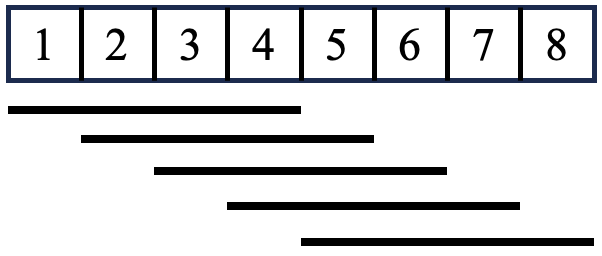
\includegraphics[scale=.24]{thesis/figures/sliding_window_left.png}}
        \caption{Shift step as one}
        \label{shift step as one}
    \end{subfigure}
    \begin{subfigure}{0.49\textwidth}
        \centering
        \adjustbox{height=3.2cm}{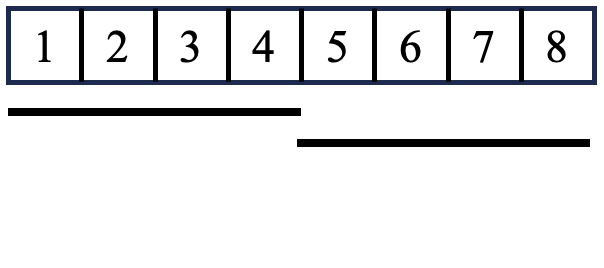
\includegraphics[scale=.24]{thesis/figures/sliding_window_right.png}}
        \caption{Stride same as the number of frames}
        \label{shift step as the fol value}
    \end{subfigure}
    \caption{Sliding window while the number of the frames is 4, where the number 1-8 represent the frames in each group and the lines illustrate the selected frames within each window.}
	\label{sliding window}
\end{figure}

According to the measurement, group and frame defined in Table \ref{recording settings}, the sliding window will only be applied to the frames, that is, sliding within each group. That is to say, the integers from 1 to 8 in Figure \ref{sliding window} above represent the pickle files stored in eight frames, namely \texttt{1.pickle} to \texttt{8.pickle}. The reason for applying it only within the group is that in the above recording setting, in order to reduce the similarity of the scenery and data, the time interval between groups and collections is larger, so only the data within each group can be regarded as continuous. The lines at the bottom of the figures represent the frames covered by the window. The four frames covered will be used as one sequence input of the model, and the data to be upsampled is the last frame within each window, and the ground truth is only the high-resolution version of this last frame.

In addition, there are two ways as shown in Figure \ref{sliding window}. The window in Figure \ref{shift step as one} moves once a step, while the window in Figure \ref{shift step as the fol value} moves according to the number of frames. Compared with the approach that only loads the certain required number of frames once within a group, the method in Figure \ref{shift step as the fol value} will obtain twice the amount of data, while Figure \ref{shift step as one} can obtain five times the amount. However, the shift method in the Figure \ref{shift step as one} will cause the overlapping part, that is, the data to be upsampled in one input also appears in another input, which blows up the scale of the dataset but doesn't bring more information. Therefore, in order to ensure the quality of the data, subsequent data processing will only use the window sliding in the way as in Figure \ref{shift step as the fol value}.

\begin{spacing}{1.5}
\textbf{\large{Resampling}}
\end{spacing}

During creating the \gls{tfrecord} files, high-resolution and low-resolution data will be stored in pairs. At this moment, the data is still in the time domain. Figure \ref{downsample in time domain with the factor of 2} draws a signal containing multiple chirps and the process of the downsampling with the factor of two.

\begin{figure}
	\centering
	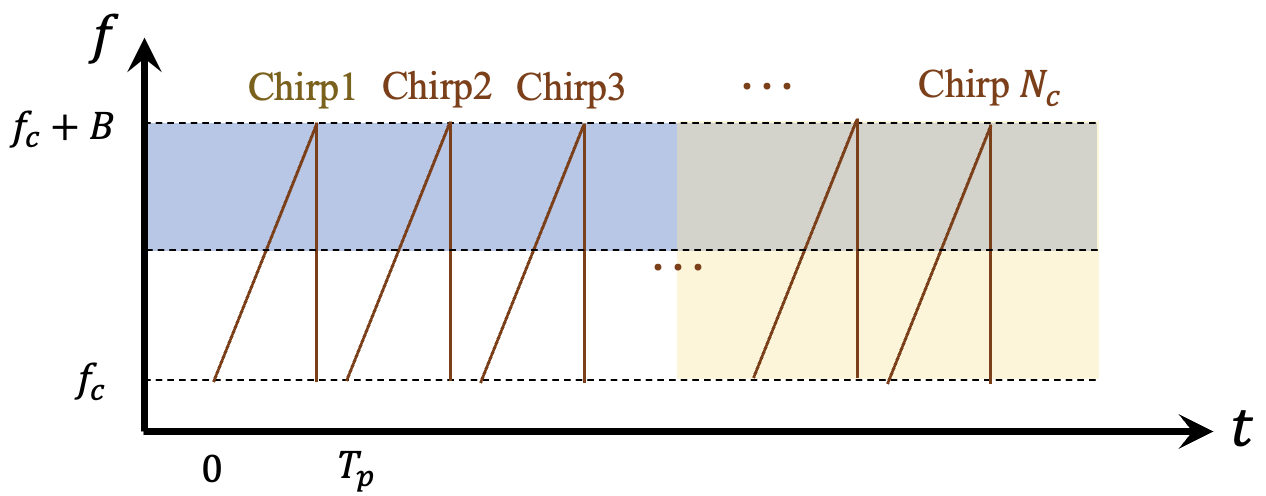
\includegraphics[scale=.67]{thesis/figures/resampling.png}
	\caption{Downsampling processing with the factor of 2 by cutting the bandwidth with only half samples within the chirp to obtain half range resolution and dropping half of the chirps to halve the velocity resolution.}
	\label{downsample in time domain with the factor of 2}
\end{figure}

Based on the radar settings selected above, the velocity and range resolutions can be calculated separately. Substituting the initial radar parameters from into the velocity resolution formula below, the value is
\begin{equation}
    \centering
    \Delta v = \frac{c}{2f\textsubscript{c}} \cdot \frac{1}{T\textsubscript{p} \cdot N\textsubscript{c}} = 0.178\,\mathrm{m/s},
    \label{velocity resolution equation}
\end{equation}

while the range resolution can be derived as
\begin{equation}
    \centering
    \Delta r = \frac{c}{2B} = 0.0375\,\mathrm{m}.
    \label{range resolution equation}
\end{equation}

First of all, regarding the resampling of velocity resolution, according to the derivation of formula \ref{velocity resolution equation}, if in order to double the velocity resolution while the speed of light and carrier frequency are constant, the \gls{cri} $T_p$ or the number of chirps $N_c$ have to be reduced to half of the original parameters. Since the \gls{cri} have the influence on the shape of chirp and it's hard to build the pairs with different \gls{cri}, the later alternative is chosen, namely the number of chirps $N_c$ turns to 32, corresponding to the abolishment of the signals under the yellow mask in Figure \ref{downsample in time domain with the factor of 2}, and only keep the first 32 chirps. In terms of the range resolution, according to formula \ref{range resolution equation}, since the speed of light is a constant, reducing the bandwidth increases the range resolution. Therefore, the blue mask in Figure \ref{downsample in time domain with the factor of 2} indicates that the upper half of the chirp has been removed, thereby halving the range resolution.

For the maximum values of both velocity and range, according to formulas \ref{maximum velocity equation} and \ref{maximum range equation}, maintaining the wavelength $\lambda$ and \gls{cri} $T_p$ can ensure that the maximum velocity is the same as the high-resolution case. When the bandwidth is reduced by half, the number of sampling points within each chirp is also reduced by half, as plugging the formula \ref{sampling frequency equation 2.6} into the formula \ref{maximum range equation}, the maximum value of the range is up to the slope only, hence, it remains.

For each high-resolution frame within the sliding window, known the shape of each high resolution data is \texttt{(64, 512)}, the pseudo-code of this downsampling process is written in Algorithm \ref{pseudo code of downsampling}.
\begin{algorithm}
    \caption{Pseudo code of resampling}
    \label{pseudo code of downsampling}
    \renewcommand{\algorithmicrequire}{\textbf{Input:}}
    \renewcommand{\algorithmicensure}{\textbf{Output:}}
    
    \begin{algorithmic}[1]
        \REQUIRE $High-resolution\ data\ as\ data,\ sampling\ rate$
        \ENSURE $Low-resolution\ data$

        \STATE $row\ =\ data.shape[0]$
        \STATE $col\ =\ data.shape[1]$
        \STATE $low\_resolution\_data\ =\ data[:row\ //\ sampling\_rate,\ :col\ //\ sampling\_rate]$
        
    \end{algorithmic}
\end{algorithm}

\begin{spacing}{1.5}
\textbf{\large{Cube de-biasing}}
\end{spacing}

During creating the \gls{tfrecord} files, another operation is cube de-biasing. Cube de-biasing refers to the mean removal of the data cube. The main purpose of this operation is to eliminate the constant offset caused by the hardware system or environment, so as to more clearly and fairly detect the reflected signal of the target, while ensuring no different offset between the chirps in the collection process.

The operation of cube de-biasing is to calculate the mean of each chirp, and then expand it to the size of $N_s$ to remove the offset along the fast time axis. The pseudo code is as following Algorithm \ref{pseudo code of cube de-biasing}.
\begin{algorithm}
    \caption{Pseudo code of cube de-biasing}
    \label{pseudo code of cube de-biasing}
    \renewcommand{\algorithmicrequire}{\textbf{Input:}}
    \renewcommand{\algorithmicensure}{\textbf{Output:}}
    
    \begin{algorithmic}[1]
        \REQUIRE $Cube\ data\ in\ time\ domain$
        \ENSURE $Debiasing\ data$

        \STATE $avgs\ =\ np.average(cube,\ 1)[:,\ None]$
        \STATE $cube\ =\ cube\ -\ avgs$
        
    \end{algorithmic}
\end{algorithm}

\begin{spacing}{1.5}
\textbf{\large{\gls{rdp}}}
\end{spacing}

After loading the \gls{tfrecord} files, one processing to do is \gls{fft}, which is used to convert the data from time domain to frequency domain. This is a very important process in radar signal processing. Decomposing the data in the time domain into different frequency components helps to provide more useful information.

But in \gls{fft}, the frequency can be positive or negative, since the sine and cosine signals in the complex component can be in both directions. However, in our radar data, the signal in time domain is real-valued, which is different from the complex-valued signal as input. The real-valued input signal has a Hermitian symmetric spectrum. The reason is that in the definition of \gls{fft}, for a discrete signal $x(n)$ with the length of $N$, its \gls{dft} conversion is as following
\begin{equation}
    \centering
    X[k] = \sum_{n=0}^{N-1} x[n] e^{-j\frac{2\pi kn}{N}}.
\end{equation}

Its conjugate is
\begin{equation}
    \centering
    X^*[k] = \sum_{n=0}^{N-1} x[n] e^{+j\frac{2\pi kn}{N}},
\end{equation}

then they both can be derived as conjugated pair, namely
\begin{equation}
    \centering
    X[N - k] = X^*[k].
\end{equation}

Therefore, there is no additional information between the positive and negative parts, in order to reduce the computational complexity and storage requirements, we can only save the information of the positive frequency part as well as one real value and discard the negative frequency part. Figure \ref{an overview of the rfft} shows well the finally obtained symmetrical data after the \gls{fft} process.

\begin{figure}
	\centering
	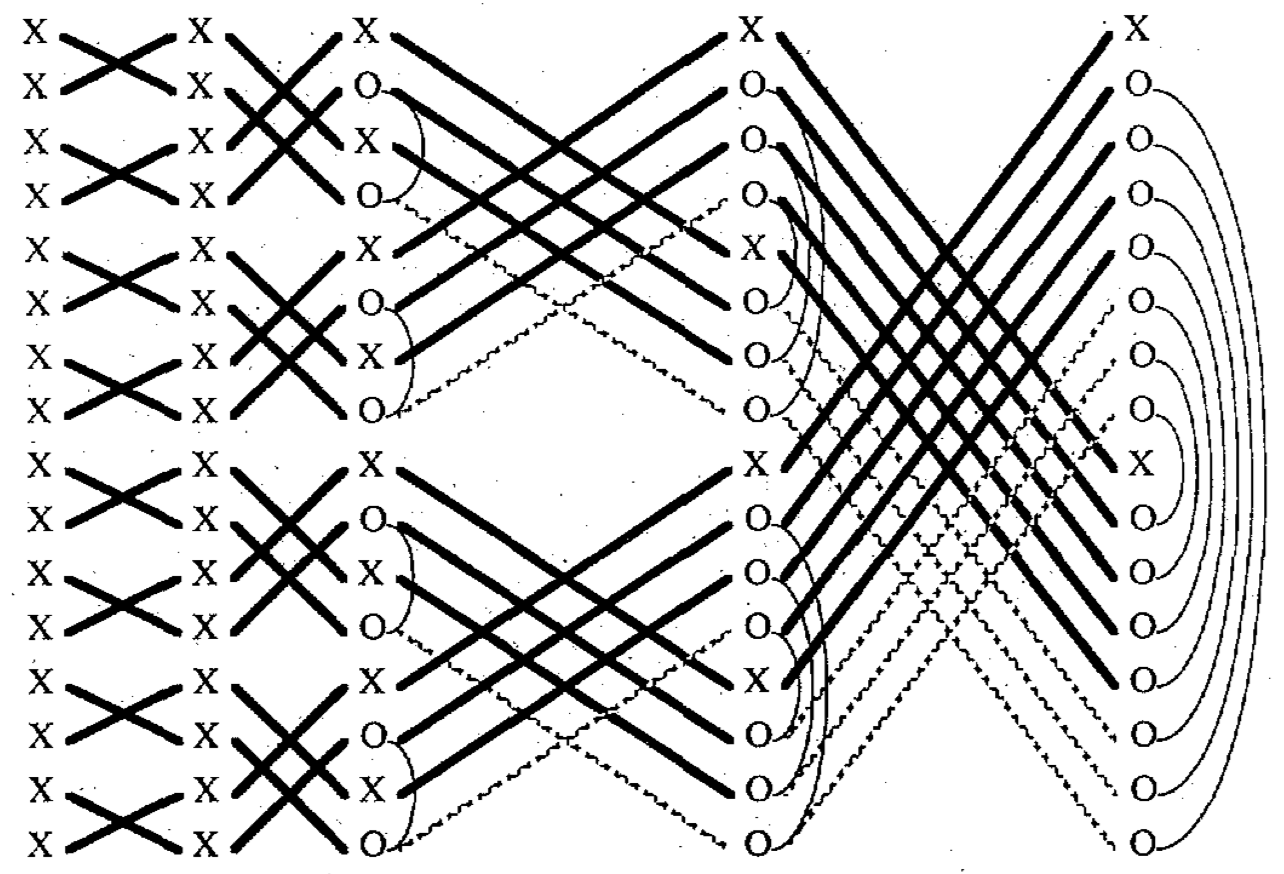
\includegraphics[scale=.45]{thesis/figures/rfft.png}
	\caption{An overview of the \gls{fft} in the case of real-valued inputs, where X indicates the real value and O represents the complex value. The figure shows the symmetric converted complex values \cite{sorensen_real-valued_1987}.}
	\label{an overview of the rfft}
\end{figure}

The data after \gls{rfft} processing contains two parts. One part is the \gls{dc} component, which can be regarded as the offset of the data and the other part is the Nyquist frequency component. In our data, when the dimension of a low resolution data obtained by double downsampling in time domain is \texttt{(256, 32)}, the dimension of the data in frequency domain will be in the shape of  \texttt{(129, 32)}, while the dimension of the low-resolution data obtained by quadruple downsampling is \texttt{(65, 16)}. Similarly, the shape of the high-resolution cube data will changed from \texttt{(512, 64)} to \texttt{(257, 64)}.

For the specific transform process, since \gls{fft} can only process time domain data of limited length, it is necessary to truncate the signal, that is, add a window, and each transform process is only performed within one window. The commonly used window functions include but not limit to the Hamming windows, Hanning windows, and blackman windows. For the two window functions built in TensorFlow, Hamming windows and Hanning windows, since the end of the Hamming window has a smaller main lobe in frequency domain which leads to a shaper range-Doppler map \cite{podder2014comparative}. Therefore, before performing \gls{rfft}, using the Hamming window function on the data cube during the \gls{rdp} is necessary.

After obtaining the windows of the range and Doppler effect axes respectively, we first apply the window on the range dimension and perform the \gls{rfft} operation. The dimension of the range will then change from 512 to 257 or from 256 to 129. The data after the \gls{rfft} operation on the range dimension is complex-valued. While applying the window on the velocity axis, it should be applied to the real and imaginary parts respectively. Since it is already complex-valued, only \gls{fft} is performed on the velocity dimension instead of \gls{rfft}. In addition, the \gls{fft} operation in TensorFlow only acts on the last dimension, so after finishing the transform on the range dimension, a transpose operation is required. Finally, since the range is between 0 and the maximum value, whereas the velocity can be in both positive and negative values, the data can be shifted so that the position where the velocity is zero centered, which is clear and convenient for the visualization. The pseudo code for this processing is shown in Algorithm \ref{pseudo code of rdp processing}.

\begin{algorithm}
    \caption{Pseudo code of \gls{rdp} processing}
    \label{pseudo code of rdp processing}
    \renewcommand{\algorithmicrequire}{\textbf{Input:}}
    \renewcommand{\algorithmicensure}{\textbf{Output:}}
    
    \begin{algorithmic}[1]
        \REQUIRE $Cube\ data\ in\ time\ domain\ as\ cube$
        \ENSURE $Range-Doppler\ map\ in\ frequency\ domain\ as\ rD$

        \STATE $range\_window\ =\ tf.signal.hamming\_window(tf.shape(cube)[2])$
        \STATE $doppler\_window\ =\ tf.signal.hamming\_window(tf.shape(cube)[1])$
        \STATE ~
        \STATE $cube\_windowed\ =\ cube\ *\ range\_window$
        \STATE $rfft\ =\ tf.signal.rfft(cube\_windowed)$
        \STATE $rfft\ =\ tf.transpose(rfft,\ perm=[0, 2, 1])$
        \STATE ~
        \STATE $re\_rfft\ =\ tf.math.real(rfft)\ *\ doppler\_window$
        \STATE $im\_rfft\ =\ tf.math.imag(rfft)\ *\ doppler\_window$
        \STATE $rfft\ =\ tf.complex(re\_rfft,\ im\_rfft)$
        \STATE $rD\ =\ tf.signal.fft(rfft)$
        \STATE ~
        \IF {$whether\_fftshift$}
            \STATE $rD\ =\ tf.signal.fftshift(rD, 2)$
        \ENDIF
        
    \end{algorithmic}
\end{algorithm}

\begin{spacing}{1.5}
\textbf{\large{\gls{irdp}}}
\end{spacing}

When the data needs to be converted from the frequency domain back to the time domain, the \gls{irdp} operation can be performed. The operation is the opposite of the above mentioned \gls{rdp} operation. First of all, make sure that the shape of each range-Doppler map is as the format of \texttt{(1, \#samples, \#chirps)}. The reason for the extra dimension at the first position is to emphasize the number of frames. The number of frames may be 4 as input, but in the output it goes to one frame. Next, use \gls{ifft} to process the velocity axis and calculate the window functions of the range dimension as well as the velocity dimension. Furthermore, since the range dimension has not yet recovered its original size, the dimension must be calculated additionally in the range window function. Then, after removing the window function in the real and imaginary parts and transposing the shape, \gls{irfft} and removing the range window function can be performed. The pseudo code is written in Algorithm \ref{pseudo code of irdp processing} as well.

\begin{algorithm}
    \caption{Pseudo code of \gls{irdp} processing}
    \label{pseudo code of irdp processing}
    \renewcommand{\algorithmicrequire}{\textbf{Input:}}
    \renewcommand{\algorithmicensure}{\textbf{Output:}}
    
    \begin{algorithmic}[1]
        \REQUIRE $Range-Doppler\ map\ in\ frequency\ domain\ as\ rD$
        \ENSURE $Cube\ data\ in\ time\ domain\ as\ cube$

        \STATE $num\_chirps\ =\ tf.shape(rD)[2]$
        \STATE $num\_samples\ =\ tf.shape(rD)[1]$
        \STATE $rD\ =\ tf.reshape(rD,\ (-1,\ num\_samples,\ num\_chirps))$
        \STATE ~
        \IF {$whether\_fftshift$}
            \STATE $rD\ =\ tf.signal.fftshift(rD, 2)$
        \ENDIF
        \STATE ~
        \STATE $rfft\ =\ tf.signal.ifft(rD)$
        \STATE $range\_window\ =\ tf.signal.hamming\_window((num\_samples-1)*2)$
        \STATE $doppler\_window\ =\ tf.signal.hamming\_window(num\_chirps)$
        \STATE ~
        \STATE $re\_rfft\ =\ tf.math.real(rfft)\ /\ doppler\_window$
        \STATE $im\_rfft\ =\ tf.math.imag(rfft)\ /\ doppler\_window$
        \STATE $rfft\ =\ tf.complex(re\_rfft,\ im\_rfft)$
        \STATE ~
        \STATE $rfft\ =\ tf.transpose(rfft,\ perm=[0, 2, 1])$
        \STATE $cube\_windowed\ =\ tf.signal.rfft(rfft)$
        \STATE $cube\ =\ cube\_windowed\ /\ range\_window$
        
    \end{algorithmic}
\end{algorithm}

\section{Pre- and post-processing of the model inputs and outputs} \label{pre- and post-processing of the model inputs and outputs}

According to the type and characteristics of the data, a more appropriate preprocessing will greatly promote the training of the model. Furthermore, the convolutional layer is common in the models. Currently, after processing by \gls{rdp}, the data is converted into complex value, whereas the convolutional layer can only be used to process the data in real value, so it needs to choose some preprocessing methods as well. In the pipeline, the following three processing steps are mainly used: the conversion from complex value to real value, that is, input data representation, the logarithm operation on the amplitude of the data, and the normalization of the data. The three processing steps contain different methods which can be combined in different ways.

\subsection{Input data representation} \label{separation types}
% real/imaginary separation
% incl. logarithm operation \& 10.0 power and cut-off to avoid the nan problem
In order to convert the range-Doppler map from complex value to real value, three different input data representations are introduced as real and imaginary representation, amplitude representation, as well as amplitude and phase representation. In addition, a very important preprocessing is about the dimensions. During the process of creating and loading \gls{tfrecord} files, mini batch dimension is introduced. Therefore, the current shape of the low-resolution data is \texttt{(batch, \#Frames, \#samples//sampling\_rate//2+1, \#chirps//sampling\_rate)}. According to the default setting of the convolutional layer in TensorFlow, the feature is always put in the last dimension, so the current data should be transposed, that is, transposed into \texttt{(batch, \#samples//sampling\_rate//2+1, \#chirps//sampling\_rate, \#Frames)}.

\begin{spacing}{1.5}
\textbf{\large{Real and imaginary representation}}
\end{spacing}

In this representation type, the real and imaginary parts of the input are taken out separately and concatenated. According to the above input size, the last dimension will be converted from \texttt{\#Frames} to \texttt{\#Frames*2}, that is, \texttt{(batch, \#samples//sampling\_rate//2+1, \#chirps//sampling\_rate, \#Frames*2)}. There are two options for the concating process. One option is to take features as the number of frames of the real part and features of the imaginary part separately and stack them directly on the last dimension, that is, \texttt{rrrriiii}, where \texttt{r} represents the real part and \texttt{i} indicates the imaginart part. Another is that separating each data and then stacking them, that is, \texttt{riririri}. After a quick experiment, we used a small model and part of the data and found that there's no big difference between these two, since the convolution is invariant to the permutation with respect to the channels. Therefore, in order to focus on more important improvements later and reduce the complexity of different combinations, the first option is used by default, that is, directly stacking the real and imaginary parts.

In this representation type, the number of kernels in the last convolutional layer in the models will be set as two, where the first dimension represents real part and the second dimension indicates imaginary part, so the final output of the model will be \texttt{(batch, \#samples//2+1, \#chirps, 2)}. While calculating the loss, this prediction is still used in this shape. Only for the visualization, the value will be considered to convert back. TensorFlow also provides a function for directly merging real and imaginary parts into a complex value.

\begin{spacing}{1.5}
\textbf{\large{Amplitude representation}}
\end{spacing}

According to the definition of range-Doppler map, there is an amplitude at the position corresponding to the range and velocity, which is a required parameter in the visualization and range-Doppler map upsampling. Therefore, a real value can be obtained by calculating the amplitude of each complex value, and the size of the input will be hence \texttt{(batch, \#samples//sampling\_rate//2+1, \#chirps//sampling\_rate, \#Frames)}.

In this case, the number of kernels in the last convolutional layer in all models will be set as 1, which represents the amplitude and the output shape would be \texttt{(batch, \#samples//2+1, \#chirps, 1)}. In the loss functions, only the difference between the amplitude can be calculated without any phase information. Meanwhile, this value is directly used while plotting the range-Doppler map, and the complex value or the signal in time domain cannot be restored.

\begin{spacing}{1.5}
\textbf{\large{Amplitude and phase representation}}
\end{spacing}

In order to retain as much information as possible, to facilitate the recovery of time domain signals and to add phase in the loss functions to supplement information, the amplitude and phase can also be concatenated. Its size will be \texttt{(batch, \#samples//sampling\_rate//2+1, \#chirps//sampling\_rate, \#Frames*2)}, and the last dimension will be concated as \texttt{aaaapppp}, where \texttt{a} represents amplitude and \texttt{p} represents phase. The output unit of the last convolutional layer in the models is 2, where the first one represents amplitude and the second dimension denotes phase.

\subsection{Logarithm operation} \label{logarithm operation}
% only in amplitude, with log10, with log2
Compared to the upsampling image or signal approaches in the state-of-art papers mentioned in section \ref{overview of the state of the art}, a significant difference is that the amplitude of our range-Doppler map in the indoor environment varies widely. As the detection range increases, the noise becomes greater and the \gls{snr} decreases. We hope that the model can also pay attention to areas with low signal power, so we need to reduce the dynamic range of the signal. One way is to perform logarithm operations on the data. For this part, there are currently two ways: no logarithm processing and logarithm processing with base 10.

\subsection{Normalization types} \label{normalization types}
% the normalisation of the input to be (-1,1) or (0,1), angle normalisation, and the global min/max/mean
In order to further reduce the dynamic range of the signal, the data can also be normalized. In addition to the amplitude, phase can also be normalized.

For amplitude normalization, there are two normalization ranges, namely (-1, 1) or (0, 1). First of all, we need to find the minimum, mean, and maximum values of the dataset. This part of the operation is performed when the \gls{tfrecord} files are reloaded but not yet converted into the mini batches. By mapping a loop in the dataset, the corresponding values can be iteratively found. The value searching and normalization operation will be performed on the training set, validation set, and test set separately, not the entire dataset. In addition, since in reality, the model can only get the low-resolution data as the input, while the high-resolution data is unknown to the model. Therefore, while calculating these values, it is based on the low-resolution data rather than the high-resolution data. Another reason is that although the data has been downsampled, the overall value range, the minimum, mean as well as maximum values and data distribution will not change much. It can be considered that the data range and distribution at low-resolution case are basically consistent with the high-resolution data.

If the range is going to be (-1,1), the normalization operation can be done by
\begin{equation}
    \centering
    \text{normalized data} = \frac{\text{data}}{\text{max}},
\end{equation}

where max means the maximum absolute value among the dataset and in case of the range (0,1), the equation should be written as
\begin{equation}
    \centering
    \text{normalized data} = \frac{\text{data - min}}{\text{max - min}}.
\end{equation}

In the case of real and imaginary representation, the normalization can be performed as 
\begin{equation}
    \centering
    \text{normalized data} = \frac{\text{data}}{\text{amplitude}}.
\end{equation}

Furthermore, since the phase is always in the range of (-\(\pi\), \(\pi\)), it can be divided by \(\pi\) to make its range fall into (-1, 1). In conclusion, the dataset can be preprocessing in these three types, and their combination can be summarized as Table \ref{combination of three different preprocessing types}.

\begin{table}
    \centering
    \caption{Combination of three different processing types, where \ding{56} represents the valid combination and - denotes no combination.}
    \label{combination of three different preprocessing types}
    \begin{tabular}{l|c|c|c}
        \hline
        \textbf{Combination} & Real/imaginary & Amplitude & Amplitude/phase\\
        \hline
        Logarithm operation & - & \ding{56} & \ding{56} \\
        \hline
        Amplitude normalization & \ding{56} & \ding{56} & \ding{56} \\
        \hline
        Angle normalization & - & - & \ding{56} \\
        \hline
    \end{tabular}
\end{table}

\section{Range-Doppler map visualization} \label{range-Doppler map visualization}
% plotting the rD map in logarithm, resolution calculation, maximum range and velocity, limit the value range of the bar.
In order to intuitively see the effect of upsampling, we can plot the range-Doppler map, which mainly includes three steps: restoring the processed part, calculating the required parameters, and drawing.

First of all, some postprocessing should be performed to reverse preprocessing, and then the parameters that need to be calculated include the amplitude of each point, range resolution, and velocity resolution. The formulas for calculating velocity and range resolution can be applied in the pipeline according to formulas \ref{velocity resolution equation} and \ref{range resolution equation}, and for the amplitude, it needs to be determined according to the input data representation. When the data is divided into real and imaginary parts, the square root of the sum of the squares should be calculated, and if it is separated by amplitude or amplitude and phase, the first value in the last dimension will be taken. In the visualization, the first range-Doppler map in the last batch of each epoch is used by default, that is, each epoch has one visualization plot. There are something also necessary to emphasize that while plotting low-resolution range-Doppler maps, the calculated resolution values must be changed according to the resampling rate. Meanwhile, since the data collected by radar device is in voltage unit, whereas the unit of range-Doppler map is in power, the above mentioned amplitude must be squared.

There are two additional settings in the range-Doppler visualization function. One is that the amplitude value can be drawn in linear scale or in dB unit. Since the data is postprocessed, the input of the visualization function is already in linear scale, but due to the large dynamic range in the data, in order to facilitate the observation of the low \gls{snr} part, the log scale is used by default, namely in dB unit. Another setting is that since the color bar in the range-Doppler map will produce different shades of colors as the amplitude in the range-Doppler map changes, in order to compare results clearly as well as according to the distribution of high-resolution data, the range in the color bar is set between -80 dB and 60 dB. When data exceeding this range exists, a warning will be displayed in logging. In the \gls{wandb} log, the corresponding low-resolution, predicted super-resolution, and high-resolution range-Doppler maps will be visualized together in this way.